% Base sur la VO 0.11.9
% Relecture technique: 
% Relecture syntaxique: 

\part{Phase de mouvement}

Durant la \emph{Phase de Mouvement}, vous avez la possibilité de déplacer vos figurines sur le champ de bataille.

\section{Étapes de la phase}

La \emph{Phase de Mouvement} est divisée en six étapes, qui doivent suivre l'ordre de la table \ref{table/etapes_mouvement}.

\begin{table}[!htbp]
\centering
\begin{tabular}{c|l}
\textbf{1} & Début du tour et de la \emph{Phase de Mouvement}. \tabularnewline
\textbf{2} & Déclaration des \emph{Charges}. \tabularnewline
\textbf{3} & Déplacement des unités en \emph{Charge}. \tabularnewline
\textbf{4} & Mouvements Obligatoires. \tabularnewline
\textbf{5} & Autres Mouvements. \tabularnewline
\textbf{6} & Fin de la \emph{Phase de Mouvement}. \tabularnewline
\end{tabular}
\caption{\label{table/etapes_mouvement}Étapes de la phase de mouvement.}
\end{table}

\section{Déclaration des charges}

Si vous voulez que l'une de vos unités engage une unité ennemie au corps à corps, vous devez d'abord lui faire déclarer une charge. Déclarez lesquelles de vos unités vont charger ce tour-ci, une par une. À chaque fois que le joueur actif déclare une charge, le joueur réactif doit déclarer une réaction pour l'unité chargée.

Une charge ne peut être déclarée que si la cible est dans le champ de vision de l'unité qui charge, et peut effectivement être chargée, c'est à dire qu'elle est à une distance inférieure à la distance maximale de charge, et qu'il y a assez de place pour amener l'unité chargeant au contact de l'unité chargée. Ne prenez pas en compte une éventuelle fuite en réaction à la charge, même si elle est obligatoire, pour vérifier si une charge est possible ou non. Prenez par contre en compte les charges déjà déclarées. Une unité ayant déclaré une charge va potentiellement bouger et ne plus gêner une autre charge.

\subsection{Réactions aux charges}

Quand une charge vient d'être déclarée contre une unité, celle-ci doit déclarer une réaction à la charge parmi les trois possibles : \emph{Tenir la Position et Tirer}, \emph{Tenir la Position}, \emph{Fuir}.

\subsubsection*{Tenir la position}

Les unités déjà engagées dans un corps à corps ne peuvent que tenir leur position. \emph{Tenir la Position} signifie que l'unité ne fait rien.

\subsubsection*{Tenir la position et tirer}

Une réaction \emph{Tenir la Position et Tirer} est possible à condition que l'unité chargée dispose d'armes de tir, que l'unité ennemie la chargeant soit dans l'arc frontal de l'unité chargée, et enfin que l'unité ennemie soit éloignée d'au moins sa valeur de Mouvement (la valeur la plus basse parmi les figurines qui chargent s'il y en a plusieurs). L'unité chargée effectue immédiatement une attaque de tir, comme elle le ferait durant la \emph{Phase de Tir}, \nouveau{et ce même si l'ennemi est au delà de la portée maximale des armes de tir utilisées}. N'oubliez pas de prendre en compte les modificateurs pour toucher appropriés, comme \emph{Longue Portée} ou \emph{Tenir la Position et Tirer}. Cette réaction à une charge ne peut être effectuée qu'une seule fois par tour, pour chaque unité réactive.

\subsubsection*{Fuir}

L'unité chargée fuit immédiatement dans la direction opposée de l'unité chargeant, en suivant la ligne droite passant par les centres des deux unités. Après qu'une unité a fait son mouvement de fuite suite à une réaction \emph{Fuir}, toutes les unités qui avaient déclaré une charge vers elle peuvent immédiatement tenter une \emph{Redirection} de leur charge. Une unité chargée mais déjà en fuite doit choisir cette réaction.

\texttt{NDT :} Pour illustrer les choix possibles de réactions, une unité peut très bien déclarer Tenir la position en réaction à une première charge, Tenir la position et tirer suite à une deuxième charge, enfin Fuir face à une troisième charge.

\subsubsection*{Rediriger une charge}

Quand une unité choisit de fuir en réaction à une charge, l'unité chargeant peut essayer de rediriger sa charge, en faisant un test de Commandement. Si elle le rate, elle doit finir sa charge vers l'unité ayant fui. Si elle le réussit, elle peut immédiatement déclarer une nouvelle charge vers une autre unité, qui pourra à son tour choisir une réaction normalement. Si plusieurs unités avaient déclaré une charge vers l'unité fuyant, chaque unité peut tenter une redirection, dans l'ordre choisi par le joueur actif. Une unité ne peut rediriger sa charge qu'une seule fois par tour. \nouveau{Toutefois, si l'unité vers laquelle la charge est redirigée fuit aussi, alors la charge peut être tentée vers l'une ou l'autre des unités en fuite. Déclarez laquelle avant de déterminer la distance de charge}.

\subsection{Déplacement des unités en charge}

Maintenant que toutes les charges et leurs réactions ont été déclarées, les unités en charge vont essayer d'atteindre leur cible. Le joueur actif choisit une unité qui a déclaré une charge et jette les dés pour déterminer la portée de charge de cette unité, puis la déplace. Répétez ce procédé pour chaque unité qui a déclaré une charge durant cette phase.

\subsubsection*{Portée de charge}

La portée de charge d'une unité est normalement sa valeur de Mouvement à laquelle on additionne 2D6. Si le résultat est égal ou supérieur à la distance entre l'unité et sa cible, on dit que la portée de charge est suffisante. L'unité peut alors faire son mouvement de charge, si elle en a la place. Si la portée de charge obtenue est strictement inférieure à la distance entre les unités, ou s'il n'y a pas assez de place pour faire le mouvement de charge, la charge est ratée. L'unité en charge doit alors faire un mouvement de charge ratée (voir plus bas).

\subsubsection*{Mouvement de charge}

Un mouvement de charge consiste à se déplacer jusqu'à entrer en contact socle à socle avec l'unité chargée. Les règles suivantes s'appliquent :
\begin{itemize}[label={-}]
\item L'unité chargeant peut avancer droit autant qu'elle le souhaite.
\item Une seule roue peut être effectuée pendant ce mouvement de charge. Cette roue ne peut dépasser un angle de 90{\text{\degree}}.
\item L'ennemi doit se trouver en contact socle à socle, avec l'avant de l'unité en charge, \nouveau{du côté de l'arc où se trouvait la majorité de l'avant de l'unité en charge quand la charge a été déclarée}.
\item L'unité en charge ignore la \emph{Règle du Pouce d'Écart}. Elle ne peut cependant entrer en contact socle à socle avec un ennemi que si elle lui a déclaré une charge.
\end{itemize}

\subsubsection*{Alignement}

Si l'unité en charge arrive à entrer en contact socle à socle, les unités doivent être alignées l'une avec l'autre, de manière à ce que leurs deux côtés soient parallèles et en contact. Tournez l'unité en charge autour du point de contact des deux unités (voir figure \ref{figure/charge}). Si cela ne suffit pas à amener les deux unités en contact complet, parce que d'autres unités ou des décors bloquent la rotation, tournez l'unité chargée à la place si cela résout le problème, \nouveau{ou encore une combinaison des deux, en tournant l'unité chargée le moins possible.} L'unité chargée ne doit être déplacée que si c'est le seul moyen d'aligner les unités. Toutefois, l'unité chargée ne peut jamais être tournée si elle était déjà engagée au corps à corps. Ces mouvements d'alignement font partie du mouvement de charge de l'unité et, de ce fait, ignorent la \emph{Règle du Pouce d'Écart}. Une unité chargée ne fait jamais de tests de terrain dangereux lors d'un mouvement d'alignement.

\subsubsection*{Maximiser le contact}

Les mouvements de charge doivent être effectués de manière à satisfaire les conditions suivantes, par ordre décroissant de priorité :

\begin{itemize}[label={-}]
\item \nouveau{Première priorité : L'unité chargée ne doit pas effectuer de rotation (voir la partie Alignement d'unités). Si la rotation de l'unité chargée est inévitable, faire pivoter cette dernière aussi peu que possible.}
\item \nouveau{Deuxième priorité : Le nombre total d'unités dans le combat doit être maximisé (notez que ceci n'est applicable que si plusieurs unités chargent la même unité).}
\item \nouveau{Troisième priorité : Le maximum de figurines des deux camps doit être en contact socle à socle avec un ennemi (en comptant celles qui peuvent faire des \emph{Attaques de soutien}.}
\end{itemize}

Du moment que toutes les conditions ci-dessus sont remplies du mieux possible, les unités qui chargent sont libres de se déplacer à leur guise (en respectant les règles des mouvements de charge).


\subsubsection*{Charger une unité en fuite}

Quand vous chargez une unité en fuite, suivez les mêmes règles pour un mouvement de charge ordinaire, sauf que vous pouvez entrer au contact de n'importe quel côté de l'unité chargée, mais aucun alignement ni maximisation ne doivent être faits. Si l'unité en charge entre en contact avec l'unité en fuite, cette dernière est retirée comme perte. L'unité en charge peut alors faire un test de Commandement. S'il est réussi, \nouveau{l'unité peut faire un \emph{Pivot Post-Combat}}.

\subsubsection*{Charges multiples}

Si plusieurs unités chargent un même ennemi, les mouvements de charge sont faits d'une manière légèrement différente. Déterminez les distances de charge de toutes les unités concernées avant de les déplacer. Une fois établi quelles unités vont atteindre la cible, faites les déplacements de charges réussies et ratées en respectant les priorités sur les unités qui parviennent au corps à corps comme expliqué dans le paragraphe \emph{Maximiser le contact}.

\subsubsection*{Charge impossible}

Quand les mouvements de charge sont effectués, une unité peut quelquefois en empêcher une autre de réussir sa charge. Quelquefois, il n'y a pas assez de place pour faire tenir toutes les unités en charge. Quand cela arrive, les unités ne peuvent plus atteindre le combat et font donc un mouvement de charge ratée.

\subsubsection*{\nouveau{Bloqué !}}

Pour éviter certaines situations d'abus où une unité ne peut pas charger une unité ennemie pourtant bien à portée et dans son champ de vision à cause d'un positionnement alambiqué des unités ennemies, appliquez la règle suivante. Si une unité ne peut pas faire une charge seulement à cause d'unités ennemies non engagées dans des corps à corps qu'elle ne pourrait pas charger normalement, elle peut faire un mouvement spécial de charge. Bougez l'unité droit devant elle, jusqu'à sa distance de charge obtenue aux dés. Si cela amène l'unité en contact avec un ennemi, ce dernier compte comme étant chargé. Au lieu de faire l'alignement normal, l'ennemi fait une \emph{Reformation de Combat} de manière à ce que les unités soient alignées l'une avec l'autre. Faites la \emph{Reformation} de façon à ce que le bon côté soit tourné vers l'ennemi.

\subsubsection*{Charge ratée}

Si une unité obtient une portée de charge insuffisante, ou si la charge est un échec pour une autre raison, l'unité fait un mouvement de charge ratée. La longueur de ce déplacement est la valeur la plus grande obtenue des dés lancés pour déterminer la portée de charge, en pouces. Faites faire une roue à l'unité, de manière à ce qu'un déplacement droit devant se fasse dans l'axe passant par le centre de l'unité et celui de sa cible, puis faites-la avancer. Ce n'est pas un mouvement de charge, donc la \emph{Règle du Pouce d'Écart} ne doit pas être ignorée. Si l'unité chargée a été détruite avant de déplacer l'unité en charge, marquez le dernier emplacement du centre de l'unité disparue et faites le mouvement vers ce point. Une unité qui a raté une charge ne peut plus bouger durant cette \emph{Phase de Mouvement} et ne peut pas tirer à la \emph{Phase de Tir} qui suit.

\begin{figure}[!htbp]
\centering
\def\svgwidth{\columnwidth}
\input{charge.pdf_tex}
\caption{a) La majorité de l'unité en charge (jaune) est dans l'arc frontal de l'unité ennemie, en vert, donc l'unité jaune doit entrer en contact avec la face avant de l'unité verte. La portée de charge nécessaire est de 1{\pouce}. \\
b) Elle avance d'abord puis fait une roue pour entrer en contact. \\
c) L'alignement se fait ensuite en tournant l'unité en charge autour du point de contact.}
\label{figure/charge}
\end{figure}

\begin{figure}[!htbp]
\centering
\def\svgwidth{\columnwidth}
\input{charge_alignement.pdf_tex}
\caption{a) L'unité violette, en charge, essaye de maximiser le nombre de figurines en contact. Cependant, les unités ne peuvent pas être alignées sans bouger l'unité verte, chargée. \\
b) Comme l'unité violette pourrait charger de manière à ce que l'unité verte ne soit pas déplacée, elle doit plutôt effectuer ce mouvement.}
\label{figure/charge_alignement}
\end{figure}

\begin{figure}[!htbp]
\centering
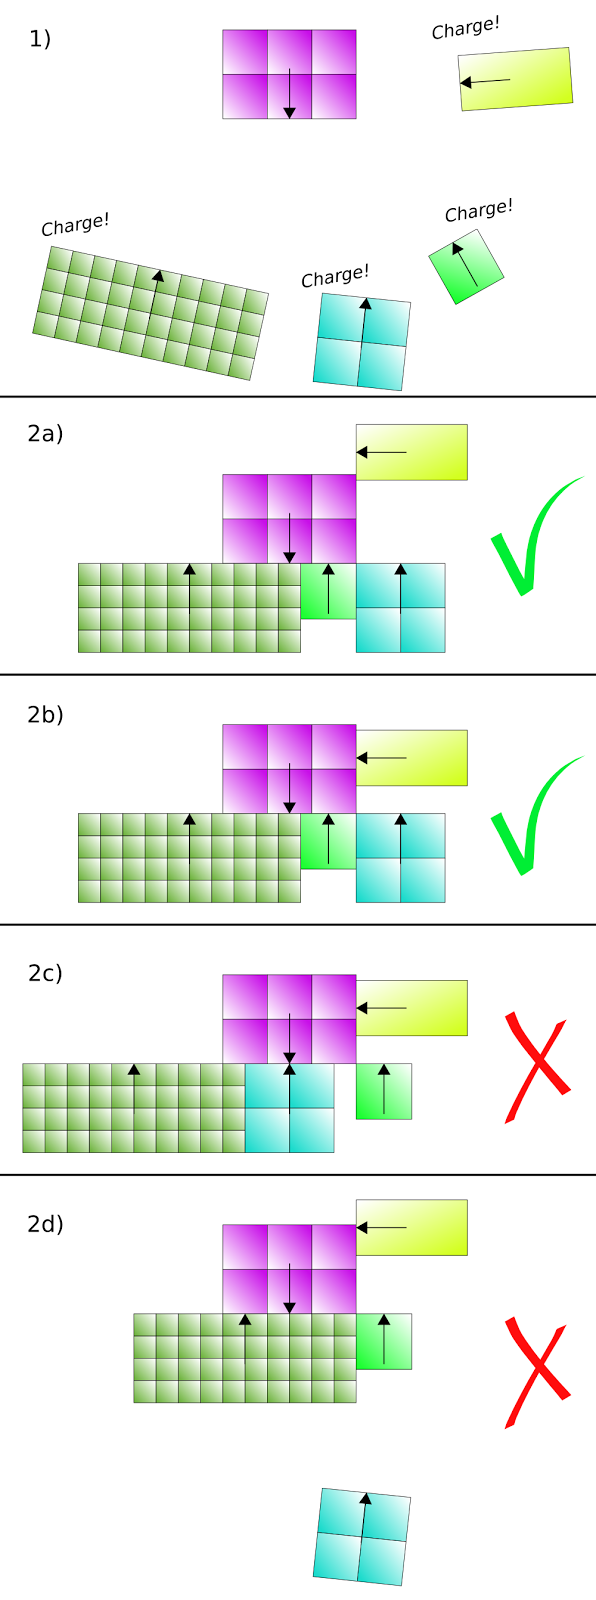
\includegraphics[width=6cm]{charges_multiples.png}
\caption{1) Des charges multiples sont déclarées contre une unité. Suivons les priorités données dans le paragraphe Maximiser le contact :\\
1. Pas de rotation.\\
2. Maximiser le nombre d'unités au combat.\\
3. Maximiser le nombre de figurine en contact socle à socle avec un ennemi.\\
\\
2a) Le nombre d'unités est maximisé (4). Une fois cette priorité respectée, le nombre de figurines en contact socle à socle doit être maximisé (12 : 8 contre 4). \\
2b) Le nombre d'unités est maximisé (4). Une fois cette priorité respectée, le nombre de figurines en contact socle à socle doit être maximisé (12 : 8 contre 4). \\
2c) Le nombre d'unités est maximisé (4). Cependant, le nombre de figurines en contact socle à socle n'est pas maximisé (10 : 6 contre 4). \\
2d) Le nombre d'unités n'est pas maximisé (3).}
\label{figure/charges_multiples}
\end{figure}

\section{Mouvements obligatoires}

Pendant cette étape de la \emph{Phase de Mouvement}, toutes les unités qui ne choisissent pas si elles vont bouger ou non, comme les unités en fuite, les unités avec un déplacement aléatoire, ou encore les unités ayant raté un test de \emph{Stupidité}, doivent bouger. Commencez par faire les tests de ralliement pour toutes les unités en fuite. Faites les mouvements appropriés suivant la réussite ou non de ces tests. Enfin, déplacez les autres unités qui bougent pendant cette étape, dans l'ordre de votre choix.

\subsection{Test de ralliement}

Au début de l'étape des \emph{Mouvements obligatoires}, toutes les unités en fuite doivent passer un test de Commandement, dans l'ordre souhaité par le joueur actif. \nouveau{Les unités qui tombent à un quart ou moins de leur effectif initial, l'effectif inscrit sur la liste d'armée, en ajoutant les \emph{Personnages} ayant rejoint l'unité, doivent faire leur test de Ralliement avec une valeur de Commandement divisée par deux, en arrondissant au supérieur.} Par exemple, prenons une unité qui a commencé la partie avec 40 figurines. S'il en reste 9, mais que 2 \emph{Personnages} ont rejoint l'unité, elle peut tout juste tenter un test de ralliement avec son Commandement non divisé. Toute unité qui réussit ce test n'est plus en fuite et peut immédiatement faire une \emph{Reformation}. Une unité qui vient de se rallier ne peut plus bouger durant cette \emph{Phase de Mouvement}, ni tirer durant la \emph{Phase de Tir} qui suit. Si le test de ralliement est raté, l'unité fait immédiatement un mouvement de fuite.

\subsection{Mouvements de fuite}

Déplacez chaque unité en fuite droit devant de 2D6{\pouce}. Si ce mouvement devait faire terminer l'unité à moins de 1{\pouce} d'une autre unité ou d'un \emph{Terrain Infranchissable}, augmentez la distance de fuite du minimum nécessaire pour éviter cette infraction. \nouveau{Si des figurines d'une unité en fuite traversent des figurines ennemies ou un \emph{Terrain Infranchissable}, elles doivent faire un test de \emph{Terrain Dangereux (3)}}. Si ce mouvement de fuite amène l'unité en contact d'un bord de table, voire le dépasse, l'unité est détruite au moment du contact, provoquant éventuellement des tests de \emph{Panique} aux unités aux alentours. Notez que ce mouvement de fuite est souvent précédé d'un pivot, qui suit les mêmes règles que le mouvement de fuite. Les mouvements de fuite ignorent tout obstacle.

\subsection{Unités en fuite}

Quand une unité fuit, elle ne peut faire aucune action volontaire. Cela inclut, par exemple, déclarer des charges, faire une réaction à une charge autre que la fuite, se déplacer d'une autre façon qu'avec un mouvement de fuite, tirer, canaliser un dé de magie, lancer des sorts, dissiper des sorts ou encore utiliser des objets à \emph{Usage Unique} qui n'ont pas besoin d'être activés. Enfin, un \emph{Général} ou un \emph{Porteur de la Grande Bannière} en fuite ne peut pas faire profiter les unités proches de leur \emph{Présence Charismatique} ou de \emph{Tenez les Rangs}.

\newpage
\section{Autres mouvements}

Les unités qui n'ont pas encore bougé durant cette phase ont l'occasion de le faire dans l'étape des \emph{Autres Mouvements}. Suivez les points de la table \ref{table/autres_mouvements} dans l'ordre.

\begin{table}[!htbp]
\centering
\begin{tabular}{c|m{12cm}}
\textbf{1} & Début de l'étape, les \emph{Renforts} arrivent. \tabularnewline
\textbf{2} & Choisissez une unité à déplacer, annoncez son type de mouvement parmi \emph{Mouvement Simple}, \emph{Marche Forcée} et \emph{Reformation}, puis bougez-la. \tabularnewline
\textbf{3} & Repassez au point 2 s'il reste des unités qui n'ont pas encore bougé et qui veulent le faire. \tabularnewline
\textbf{4} & Fin de l'étape. \tabularnewline
\end{tabular}
\caption{\label{table/autres_mouvements}Étapes des Autres Mouvements.}
\end{table}

\subsection{Mouvement simple}

Pendant un \emph{Mouvement Simple}, une unité peut avancer, reculer ou faire des pas de côté. Elle ne peut pas combiner ces directions. Les unités composées d'une seule figurine peuvent toujours faire autant de pivots qu'elles le souhaitent pendant un \emph{Mouvement Simple}. \newrule{Aucune figurine d'une unité effectuant un \emph{Mouvement Simple} ne peut se déplacer au delà de sa valeur de mouvement (depuis sa position initiale). Si le déplacement fait partie d'une \emph{Reformation Rapide}, la distance est mesurée depuis la position après la \emph{Reformation}}.

Quand elle avance, une unité peut le faire sur une distance maximale de sa caractéristique de Mouvement, en pouces. Elle peut faire autant de roues qu'elle le désire pendant le mouvement. Quand elle recule ou qu'elle fait des pas de côté, la distance maximale est \nouveau{la moitié de sa caractéristique de Mouvement}. L'unité ne peut alors pas faire de roue.

\subsection{Marche forcée}

Pendant une \emph{Marche Forcée}, une unité ne peut qu'avancer, et sur une distance maximale de deux fois sa caractéristique de Mouvement, en pouces. Elle peut faire autant de roues qu'elle le souhaite.\newrule{Aucune figurine d'une unité effectuant une \emph{Marche Forcée} ne peut se déplacer au delà du double de sa valeur de mouvement (depuis sa position initiale).}

Si des unités ennemies se trouvent à moins de 8{\pouce} de l'unité voulant faire une \emph{Marche Forcée} (avant de la bouger), cette dernière doit faire un test de \emph{Marche Forcée}. Faites un test de Commandement. S'il est réussi, l'unité peut faire une \emph{Marche Forcée} normalement. Sinon, l'unité doit fait une \emph{Marche Forcée} avec une pénalité de mouvement, la distance maximale est sa caractéristique de Mouvement. Une unité qui a fait une \emph{Marche Forcée} ne peut pas tirer dans la \emph{Phase de Tir} qui suit. Une unité composée d'une figurine seule peut faire autant de pivots qu'elle le souhaite durant sa \emph{Marche Forcée}.

\subsection{Reformation}

Repérez le centre de l'unité, puis retirez l'unité du champ de bataille. Vous pouvez la replacer dans n'importe quelle formation autorisée et orientée suivant n'importe quelle direction, en suivant bien sûr la \emph{Règle du Pouce d'Écart}, tant que son centre reste à l'emplacement repéré. Après la \emph{Reformation}, aucune figurine ne peut se retrouver plus loin de sa position originelle que deux fois la valeur de son Mouvement. Une unité qui a fait une \emph{Reformation} ne peut pas tirer dans la \emph{Phase de Tir} qui suit.

\section{Pivots et roues}

Un \emph{Pivot} est pratiqué principalement par les figurines seules. Pour faire un \emph{Pivot}, repérez le centre de l'unité, et \nouveau{retirez l'unité du champ de bataille. Replacez là ensuite dans la même formation, orientée dans la direction de votre choix, avec son centre toujours à l'emplacement repéré. Suivez normalement la \emph{Règle du Pouce d'Écart}}. 
Quand une unité fait une \emph{Roue}, tournez l'unité autour d'un de ses coins avant (\newrule{N'oubliez pas que l'unité doit avancer)}. La distance parcourue par l'unité correspond à celle parcourue par la figurine du coin avant opposé. \newrule{On considère que toutes les figurines de l'unité ont parcouru cette distance.}

\begin{figure}[!htbp]
\centering
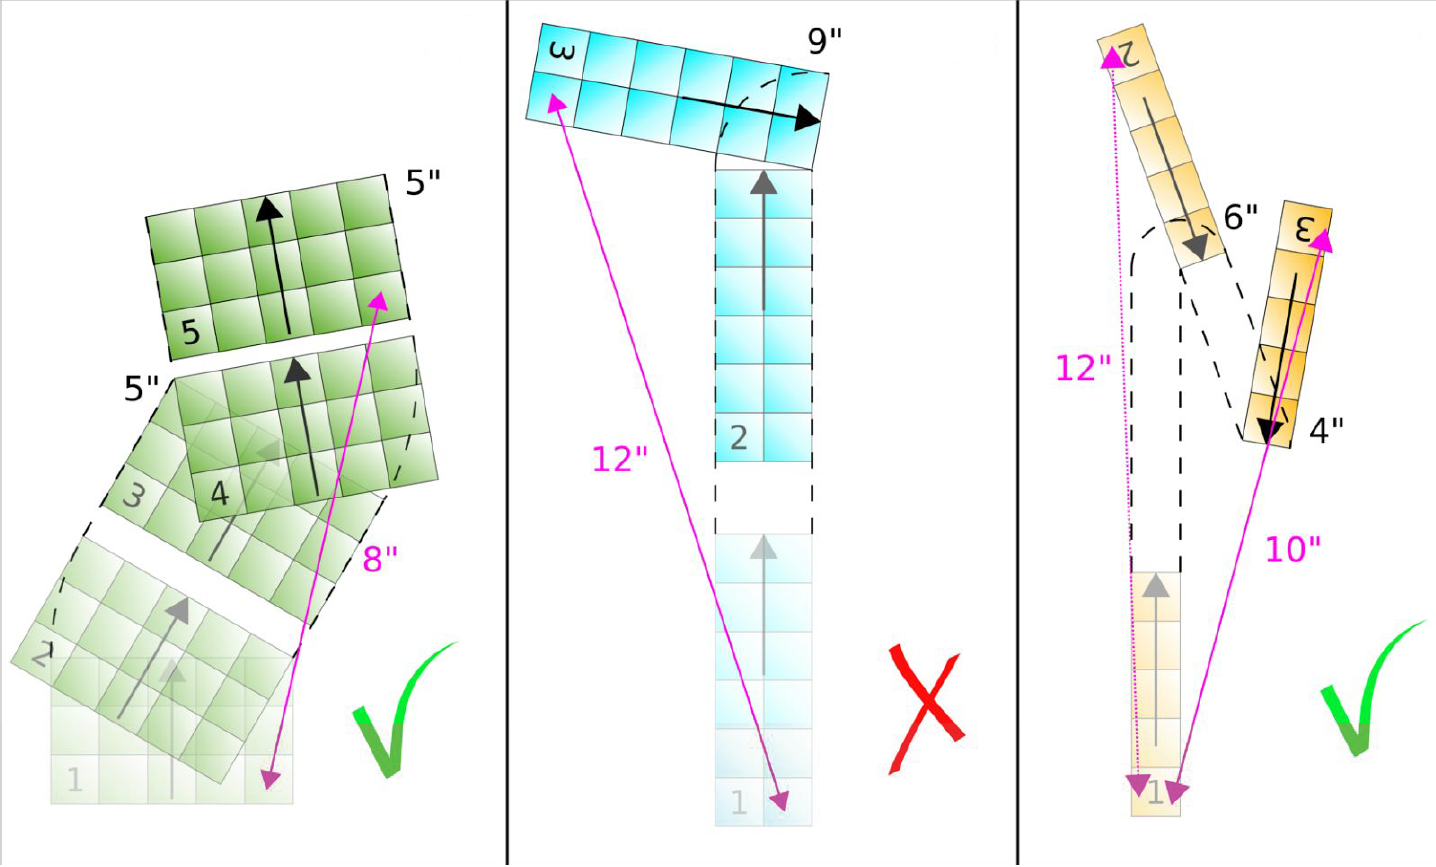
\includegraphics[width=15.5cm]{roue.png}
\caption{Les unités de cet exemple ont toutes un Mouvement de 5. \\
L'unité verte fait deux \emph{Roues} pendant une \emph{Marche Forcée}. L'unité compte comme ayant bougé de 10{\pouce}, puisque la mesure de distance est prise au niveau du coin opposé au coin qui sert de point de rotation. \\
L'unité turquoise fait une \emph{Roue} pendant une \emph{Marche Forcée}. Cependant, ce mouvement est non réglementaire, car même si la figurine du coin opposé n'a bougé que de 10{\pouce}, certaines figurines de l'unité se sont déplacées de plus de 10{\pouce}. \\
L'unité jaune fait une \emph{Roue} pendant une \emph{Marche Forcée}. Elle compte comme ayant bougé de 10{\pouce}, puisque la mesure de distance est prise au niveau du coin opposé au coin qui sert de point de rotation. Remarquez qu'aucune figurine n'a bougé de plus de 10{\pouce} depuis sa position initiale.}
\label{figure/roue}
\end{figure}
